\documentclass[12pt]{scrreprt} 
\usepackage{tikz}
\usepackage{caption}
\usepackage[margin=1in,bmargin=1in,lmargin=1in,rmargin=1in]{geometry}
\usepackage{setspace}
\usepackage[style=mla, noremoteinfo=true]{biblatex}
\usepackage{hyperref}
\usepackage[american]{babel}
\usepackage{csquotes}

\renewcommand*{\pagemark}{}

\usepackage{fancyhdr}
\fancypagestyle{plain}{%
\fancyhf{}
\fancyhead[R]{Allen \thepage}
\fancyfoot{}
\fancyfoot[C]{}
\renewcommand{\headrulewidth}{0pt}
\renewcommand{\footrulewidth}{0pt}}

\pagestyle{plain}

\renewcommand*{\chapterheadstartvskip}{\vspace*{1cm}}
\renewcommand*{\chapterheadendvskip}{\vspace*{2cm}}

%titlesec: chapter/section package to manipulate sections
\usepackage{titlesec}
\titleformat{\chapter}[block]
	{\normalfont\bfseries\filright}{\thechapter}{12pt}{}
\titleformat{\section}[block]
	{\normalfont\bfseries\filright}{\thesection}{12pt}{}
\titleformat{\subsection}[block]
	{\normalfont\bfseries\filright}{\thesubsection}{12pt}{}
\titlespacing*{\chapter}{0pt}{10pt}{10pt}

\addbibresource{a15.bib}
\doublespacing
\captionsetup[figure]{labelformat=empty}

%\usetikzlibrary{automata,positioning}
%\PassOptionsToPackage{usenames,dvipsnames,svgnames}{xcolor}


\begin{document} 

\begin{titlepage}

\newcommand{\HRule}{\rule{\linewidth}{0.5mm}} % Defines a new command for the horizontal lines, change thickness here

\center % Center everything on the page

%----------------------------------------------------------------------------------------
%	HEADING SECTIONS
%----------------------------------------------------------------------------------------

\textsc{\LARGE University of North Alabama}\\[1.5cm] % Name of your university/college
\textsc{\Large Computer Architecture and Organization}\\[0.5cm] % Major heading such as course name

%----------------------------------------------------------------------------------------
%	TITLE SECTION
%----------------------------------------------------------------------------------------

\HRule \\[0.4cm]
{ \huge \bfseries Cortex A15 Processor}\\[0.4cm] % Title of your document
\HRule \\[1.5cm]
 
%----------------------------------------------------------------------------------------
%	AUTHOR SECTION
%----------------------------------------------------------------------------------------

\begin{minipage}{0.4\textwidth}
\begin{flushleft} \large
\emph{Author:}\\
Jeffrey \textsc{Allen}
\end{flushleft}
\end{minipage}
~
\begin{minipage}{0.4\textwidth}
\begin{flushright} \large
\emph{Professor:} \\
Dr. Patricia \textsc{Roden}
\end{flushright}
\end{minipage}\\[4cm]

{\large \today}\\[3cm] % Date, change the \today to a set date if you want to be precise

\vfill % Fill the rest of the page with whitespace

\end{titlepage}

\tableofcontents

\pagebreak
\begin{flushleft}
Jeffrey Allen\\
Dr. Patricia Roden\\
Computer Science 311\\
22 October 2014
\end{flushleft}

\centerline{Cortex A15 Processor}

{\let\clearpage\relax\chapter{History}}

% Describe very beginning
In 1985, the Acorn Computer Group birthed the ARM architecture in the United Kingdom. This was only the beginning to the quick pace ARM began developing and evolving their architectural designs. Two short years afterwards, Acorn released its first RISC processor that was optimized for low-cost personal computers. Following this, in 1990, ARM which originally stood for Acorn RISC Machine developed its Advanced RISC Machines. This design defined its 32-bit RISC-like architecture generally used today.

	% Describe middle to end in one paragraph
	According to Linda Null and Julia Lobur there are multiple families of ARM architectures and processors \autocite[327]{classtext}.
	The problem domain which the processor is designed for group them into these different families. 
	These architectures include include the ARM1, ARM2, which span to the ARM11 architecture.
	The processors are also categorized into different "series".
	ARM supports the M series, R series, and A series.
	The M series processors are optimized for microcontrollers. 
	The R series has been designed for embedded systems and real time applications.
	Whereas the A series, which includes the A15, has been designed to handle full operating systems in third party applications. 
	It can be implicitly understood by the name that the A15 was designed and optimized for the latter domain.

{\let\clearpage\relax\chapter{Instruction Sets}}

		I'll begin this section with explaining that an interface is an intermediary between two entities.
	Humans have utilized this concept in order to build rockets which have reached mars, create heart rate monitors, and even predict weather. 
	A computer's processor is only designed to fetch, decode and execute various instructions.
	Before all of that, it must first be able to understand what its supposed to do.
	Since humans and computers are worlds apart when it comes to communicating with each other, the Instruction Set Architecture (ISA) interface was created.
	This interface saves humans from learning the exact strings of 0's and 1's the processor understands in order to carry out an instruction.
	Essentially, this is the agreed-upon interface designed for a machine allows software to able to communicate with the hardware that executes it\autocite[233]{classtext}.

	\section{RISC Vs. CISC}
	% Dandamudi example pg 5
	There are two types of processor design philosophies \autocite[5]{riscGuide}. One of them is the RISC, or the Reduced Instruction Set Computer design. The other is CISC, or the Complex Instruction Set Computers design. CISC systems can be described through an example. Subtracting two integers is considered "simple". Then there is a type of instruction which can be categorized as complex, which can be found in a bubble sort swap routine.

	
	Bubble sort essentially sorts a list by taking an array $ A $, copying one element $ \alpha $ located at index $ A_{x} $ and "bubbles" it up it its correct position.
	When another element $\beta$ located at $ A_{y} $ found to be the $ \alpha $'s correct position, the complex swap instruction begins.
	In the interest of not losing $\beta$, we must first copy it into a temporary location, which then allows $\alpha$ to be inserted into it.
	After that, $\beta$ can safely be stored into $\alpha$'s original position.
	CISC systems are based off of these complex instructions that performed multiple operations in a single instruction.
	These instructions were used primarily in the 1950's through the 1970's and early 1980's.
	This is because of the limitations of memory and cost ( 16KB of memory $\approx$ \textdollar500 ) which architecture designers were able to optimize all instructions for a specific task.

	% Class Text / Dandamudi
	RISC systems were designed with simplicity in mind.
	This is achieved by keeping all instructions small in order to execute the more efficiently.
	A notable difference between the two philosophies is that RISC assumes that required operands are not in memory, but directly in the processor's internal registers.

	\section{Main ISA: ARMv7-A}

	At the end of the day, it is all about communication.
	Moore's Law, states that the density of transistors on an integrated circuit is doubling every 18 months.
	This law explains one of the main reasons why communication between humans and computers has changed, and continues to change so rapidly.
	The concept applied to the range of years between 1960 to 2014 describes a fair amount exponential increase in transistors, or rather, methods of communication.
	As Linda Null and Julia Lobur point out though, RISC in today's society something of a misnomer \autocite[327]{classtext}.
	They say that almost all recently created instruction sets are a mixture of RISC's and CISC's.
	It can be seen in practice with the Cortex-A15 which supports its main ARMv7-A architecture, supplemented with the Thumb, Advanced SIMD, and VFP architectures.

	\section{Extentions to ARMv7-A Instructions}

	Being that the A15 is the fourth generation of processors designed by ARM, it has evolved extensively.
	Good designs are kept and streamlined, while the bad died out.
	To keep up with the evolution of computation the A series began to be designed with ability to decode different instruction sets. 
	Depending on what state, or "\textit{CPU Mode}", of operation of execution the processor is in, will determine how the instruction will be translated.
	The state indication is controlled by a simple switch of the designated T (Thumb) bit and J (Java) bit in the processor's Current Program Status Register (CSPR).
	This will be explained later in the "Registers" section.
	With the A15 having the ability to support multiple ISA's, this allows for is the Large Physical Address Extension (LPAE) architecture to enable virtual environments.

	Why have support for virtual environments though? 
	As stated before, the Cortex-A series is a family of processors which is only evolving with the times.
	More and more computation must be supported, so a processor needs to be versatile enough to keep up with the designs.
	The A series supports multiple instruction sets, or extensions of them, in order to live on.
	These include the ARMv7-A, Thumb, ThumbEE, NEON, and VFP instruction sets. 
	ARM's A15 reference manual indicates on various occasions when to refer to other documentation sources to describe it's own features.

		\subsection{Thumb \& ThumbEE}
			This instruction set basically truncates the most commonly used 32-bit ARM instructions into 16-bit instructions.
			Therefore, creating even simpler instructions that are executed more efficiently.

		\subsection{Jazelle}
			This instruction set executes \textit{Java bytecode}.
			Java is a high-level programming language which was designed to be portable.
			Portability is achieved by embedding machines with a JVM (Java Virtual Machine).
			This virtual environment translates the byte code into machine specific instructions which it is executed upon.
			
		\subsection{Advanced SIMD (Single Instruction Multiple Data)}
			The advanced SIMD extension is a media and signal processing architecture.
			This set of instructions adds the functionality targeted primarily at audio, video, 3-D, graphics, image, and speech processing.
		
		\subsection{VFP (Vector Floating Point Co processor Extension) \& NEON}
			In essence, all these instruction sets are designed to do is make computation highly efficient.
			As stated in the A15 manual, the NEON technology provides support for integer and floating-point vector operations.
			While the VFP extension performs single-precision and double-precision floating-point operations.
			These instructions both support all addressing modes, data types, and operations provided by the Advanced SIMDv2 extension as well.

{\let\clearpage\relax\chapter{Memory Specifications}}

	Memory in the ARM architecture models memory as a single array of $2^{32}$ 8-bit bytes.
	In total, that is 4,294,967,296 bytes of memory (or 34,359,738,368 bits. Whoo. That's quite alot to take care of). In reviewing the ARM Architecture Reference Manual ARMv7-A and ARMv7-R edition, the list of following data types are supported in memory:

	% Chapter 14 in Cortex A15 technical reference manual (file : ./ArmCortex15_manual.pdf)
	% A2.2 ARMv7 manual.

	\begin{center}
		\begin{tabular}{|l|l|}
		\hline
			\bfseries Byte & 8 bits \\ \hline
			\bfseries Halfword & 16 bits \\ \hline
			\bfseries Word & 32 bits \\ \hline
			\bfseries Double word & 64 bits \\ \hline
		\end{tabular}
	\end{center}

	Unsigned numbers represent byte addresses that range from 0 to $2^{32}-1$.
	Word-aligned addresses are divisible by 4.
	While halfword-aligned addresses which are divisible by 2.
	The blessing and curse associated with the A15 is that it supports unaligned memory storage as well.
	This gives a programmer just enough rope to hang him or herself if not careful enough to read the SCTLR (System Control Register) documentation associated with this method of memory access.

	Load and store operations are able to transfer bytes, halfwords, or words to and from memory.
	The loading of bytes or halfwords zero-extend (pad with zeros) or sign-extend (increasing number of bits of a binary number while preserving the number's sign and value) the data as it is loaded, or specified by the load instruction.

	%3.8.1 
	The A15's ARM instructions are word-aligned .
	This means the address of memory an instruction is allowed access must be divisible by 4.
	Since multiple instruction sets are supported, it is wise to mention that Thumb instructions are halfword-aligned.
	As for Java byte-code instructions, they are simply be byte aligned.
	This means it has no real limitations of where memory addresses can be accessed.
	Unaligned memory is supported with special instructions with ARMv7's instruction set.

{\let\clearpage\relax\chapter{Instruction Format}}

	% check out programmer's model in chapter 3 (file : ./ArmCortex15_manual.pdf)
	Since the ARMv7-A architecture is based off of the RISC design, all instructions are the same size.
	The Cortex A15 extends this base ARMv7-A architecture to support the Thumb instruction set though \autocite[3-2]{a15man}.
	This allows 16 bit instructions to be executed as well.
	For example, this can omit a 4-bit condition code field that is set to indicate how an instruction must be executed in certain situations.
	Figure 1 is a visual representation of what these instructions look like.
	
	\begin{figure}[h]
		\centering
			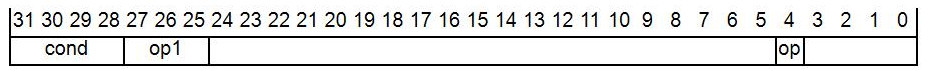
\includegraphics[width=0.7\textwidth]{croppedIE}
		\caption{Figure 1}
	\end{figure}

	% ARMv7 reference manual pg. A2-53/A3-111
	% Explanation came from book
	\section{Endianess}
	In the many layers of abstraction that exist in a computer, the endianness of an architecture must be carefully taken into consideration.
	The endianess of an architecture refers to the "byte order" of the computer.
	This can also be explained as the method of which a computer stores multiple-byte data elements.
	For example, the 4-bit string made up of $2$ 2-bit data elements $0001$, can be read by a computer in little-endian as $4_{10}$. 
	Alternatively, read as big-endian it would be $1_{10}$.
	The ARMv7-A architecture exclusively exhibits little-endian practices \autocite[A2-53]{a7man}.
	The A15 however, has an interesting but dangerous characteristic which gives it the ability to configure itself between little-endian or big-endian.
	Through the use of ARM and Thumb instruction $SETEND$ $BE$ which translates to 0, or $SETEN$ $LE$ which translates to 1 to decipher which endinaness must be observed.

	\section{Data Transfer Instructions}
	Load and store instructions are utilized to move data from registers to memory.

	\subsection{Moving}
	Being that the Von Neumann model is the architecture many computers today utilize, it is imperative for computers to be able access data in storage.
	This is where the difference in word, halfword, and byte addressable instructions come into play.
	Flags are set in the CPSR if an instruction tries to illegally access data.
	This method of exception handling has worked quite well for ARM since it has been around for close to 30 years.

	\subsection{Arithmetic}
		Add, subtract, and multiply instructions are supported by the ARMv7A architecture.
	\subsection{Comparison}
		This is also known as logical and bit instructions.
	\subsection{Branch}
		Instructions of this type all manipulate the control flow of a program.
		This includes instructions such as $BL$ which will which branch with a link back to the original program.
	\subsection{Stack Operations}
		It can be seen with the complex $STM$ instruction that more than one operation is being executed.
		With the help of register 13, the stack pointer allows for this instruction treat the registers as a stack and push multiple sets of data onto it.

	The ARM instruction and Thumb instruction reference guides are located in the appendix.

{\let\clearpage\relax\chapter{Registers}}
%\chapter{Registers}

	Essentially, a register is a place on the processor where data, instructions and state information is held.
	At any given moment in time, the A15 is said to have access to 16 of these high speed memory locations which are 32-bits wide.
	Drawing from the concepts introduced in chapter 3, the need for virtualization is essential to todays computing standards.
	The different modes of execution supported by the A15 allows for this small set of 16 groups of registers to actually be viewed as having a total of 37 groups.
	There are exactly 7 of these different modes which are subdivided further into either a \textit{User} mode, or \textit{Privileged} mode.
	
	Modes of execution can be explained by example.
	Not everyone in the United States of America has the privileged to round up its armed forces to invade another country.
	A repeat-offense criminal instructing a powerful fleet of soldiers ready to go to war is quite different from a decorated five star general being in command.
	If the army didn't follow necessary precautions and protocols to check who was in charge of it, we would simply have world chaos.
	In order to relate this back to the topic at hand, I view the A15 processor as that powerful American fleet of troops which fortunately review their instructions before being executed.
	Different processing modes allow the processor to put restrictions on the instructions it is executing.

	These multiple instruction sets and modes supported by the A15 heavily influenced the design of its registers.
	The A15 manual often times references various other manuals to describe its own details.
	Due to the wide variety of references the A15 manual uses to describe its registers, I will only be explaining how its main instruction architecture utilizes these registers.
	Figure 2 describe these 15 groups registers.

	\begin{figure}[h]
		\centering
			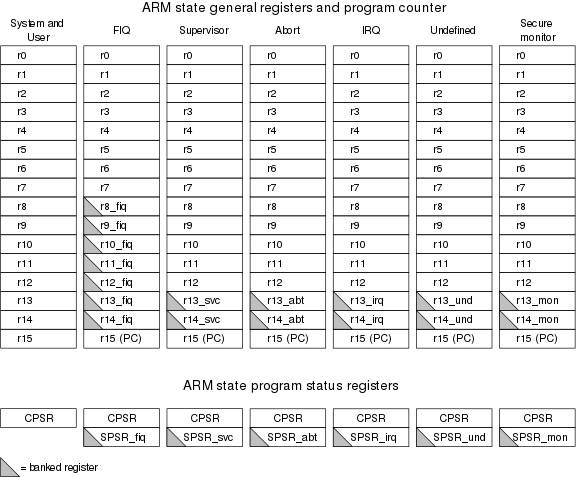
\includegraphics[width=0.6\textwidth]{registers}
		\caption{Figure 2}
	\end{figure}

	The multiple columns distinguish which state the processor is in.
	The rows situated under each column represent how the processor views each register.
	Registers labeled unbanked are able to be accessed from all processing modes.
	This means that these registers can manipulated by however they see fit.
	As for the banked registers, they have access to registers which contain sensitive system data.

	Registers 13 through 15 can be easily described as containing this sensitive data \autocite[A2-45]{a7man}.
	These 3 groups of registers are reserved for being the stack pointer registers, link registers, and program counter respectively.
	When manipulated incorrectly, personal security, hardware damage, and other various devastating events may occur.
	Referring back to the example of the common criminal opposed to the general being in command, it can be seen why different modes exists.

	The user mode is the only unprivileged mode in the A15.
	This is where the general purpose registers 0-7 can be manipulated at will.
	Application programs are usually run under these set of conditions.
	As for the other five, registers 8-12, they are all banked registers \autocite[123]{riscGuide}.

	For further reading acronym definitions are, Sivarama P. Dandamudi does a beautiful job explaining these terms in his book, \textit{"\underline{Guide to RISC Processors}"}.

{\let\clearpage\relax\chapter{Data Types}}

	\section{Register Data Types}

	\begin{itemize}
		\item{32-bit pointers}
		\item{Unsigned or signed 32-bit integers}
		\item{Unsigned 16-bit or 8-bit integers, held in zero-extended form}
		\item{Signed 16-bit or 8-bit integers, held in sign-extended form}
		\item{Two 16-bit integers packed into a register}
		\item{Four 8-bit integers packed into a register}
		\item{Unsigned or signed 64-bit integers held in two registers}
	\end{itemize}

	Unsigned, according to this processor's specification manual, is described as a data value representing a non-negative integer in the range $0$ to $2^{N-1}$.

	\section{Pseudo-Instruction Data Types}

	Pseudo instructions are instructions that are written specifically for the ARM's assembler.
	This is just another interface which programmers utilize to write code which translates to the appropriate combination of ARM or Thumb instructions.
	The translation of these pseudo-instructions occurs during the assembly time.
	These instructions support:

	\begin{itemize}
		\item{Bitstring}
		\item{Integer}
		\item{Boolean}
		\item{Real}
		\item{Enumeration}
		\item{List}
		\item{Array}
	\end{itemize}


{\let\clearpage\relax\chapter{Addressing Modes}}

	Addressing modes allow us to specify where instruction operands are located.
	Without addressing modes, it would not be possible access data because the computer wouldn't know where to seek the information.
	There are different methods in which the address in memory is generated by the load or store instructions.
	Again, the rigorous documentation would exceed the scope of this paper, so only general addressing modes will be introduced.
	
	\section{Offset addressing}
		This method specifies an offset value which is applied to an address gathered from the base register.
		The result of this is then used as the address for the instruction to fetch.
		It is noteworthy to say the base register remains unchanged.

	\section{Pre-indexed addressing}
		In the ARMv7A reference manual \autocite{a7man}, it describes this method of addressing as follows:
		"The offset value here is applied to an address obtained from the base register.
		The result is used as the address for the memory access, and written back into the base register."

	\section{Post-indexed addressing}
		The address obtained from the base register is used as the address for memory retrieval.
		After this, the offset value is then applied to the base register

In each mode of addressing, all rules of alignment and endianess applies.

{\let\clearpage\relax\chapter{Unusual Features}}

	It was previously stated that not all recent computers completely encompass one principle.
	With the versatility the A15 portrays, it is only natural that I found instructions that do not follow the RISC philosophy.
	It is seen with the $ldm$ instruction that it can execute multiple operations with one instruction.

{\let\clearpage\relax\chapter{Major Contribution to Architecture Design: Low Energy Computing}}

	The ENIAC was the first all-electronic, general-purpose digital computer.
	In 1946, this machine used 17,468 vacuum tubes that malfunctioned roughly every 20 hours which spanned 1800 square feet of warehouse space.
	This 30 ton machine that ate 174 kilowatts of power had a single processor which ran at 0.1 Hz.
	All of these facts become somewhat of a joke compared to the A15 processor.
	The A15 is being outfitted in todays mobile smart phones and calculators which fit in the back pocket of a pair of Levi jeans.
	
	The \textit{big.LITTLE} architecture developed by ARM is one of the key components behind how low energy computing is achieved.
	As seen throughout this text, ARM has the ability to combine systems seamlessly.
	In 2011, ARM revealed a design claiming it to be "The Most Energy Efficient Application Processor Ever".
	The architecture coupled the Cortex A7 processor with the Cortex A15 processor.
	Coupling these two processors together in the same system opened up the option for assigning tasks more efficiently.

	The A15 is the clear winner when it comes to high performance processing power.
	However, high battery power consumption is the price to pay to support this.
	The A7 processor specs are sub par compared to the A15, but this is good because idle states consume less energy.
	This driving concept of assigning processing intensive tasks to the A15 while applications that require less processing power utilize the A7 for its computing needs.

	Clearly, it can be seen why the A15 processor is classified as the \textit{big} component of the architecture.
	It's computing power is unparalleled to its predecessor.
	However, the A7 cannot be counted out because it consumes much less energy to power itself.

{\let\clearpage\relax\chapter{Uses/Applications: Mobile Computing}}

	% Interview with Steve Furber. ACM digital library pdf.
	Ph.D. Steve Furber, one of the principal designers of the BBC Microcomputer System and ARM microprocessors when the "A" in ARM stood for "Acorn", had this to say when interviewed by Jason Fitzpatrick \autocite[1]{steveFurber}. "The ARM architecture is the most widely used 32-bit RISC architecture and the ARM processor's power efficiency performing the same amount of work as other 32-bit processors while consuming one-tenth the amount of electricity has resulted in the widespread dominant use of the ARM processor in mobile devices and embedded systems." This whole research paper is based off of fascination related to ubiquitous computing. So when I decided to conduct research on what was behind the popular Samsung's Galaxy S4 successful mobile phone design, it was not a coincidence to find out it was ARM behind the processor design.

\printbibliography
\end{document}